\documentclass[conference]{IEEEtran}
\IEEEoverridecommandlockouts

\usepackage{cite}
\usepackage{amsmath,amssymb,amsfonts}
\usepackage{algorithmic}
\usepackage{graphicx}
\usepackage{textcomp}
\usepackage{xcolor}
\usepackage{url}
\usepackage{booktabs}
\def\BibTeX{{\rm B\kern-.05em{\sc i\kern-.025em b}\kern-.08em
    T\kern-.1667em\lower.7ex\hbox{E}\kern-.125emX}}

\makeatletter
\newcommand{\linebreakand}{%
  \end{@IEEEauthorhalign}
  \hfill\mbox{}\par
  \mbox{}\hfill\begin{@IEEEauthorhalign}
}
\makeatother

\begin{document}

\title{An Integrated AIOps Framework for Predictive Failure Detection and Autonomous Resource Optimization in CI/CD Pipelines}

\author{
    \IEEEauthorblockN{Tejas A. Jagtap}
    \IEEEauthorblockA{\textit{Department of Computer Science and Engineering} \\
    \textit{COEP Technological University}\\
    Pune, India\\
    jagtapta24.comp@coeptech.ac.in}
    \and
    \IEEEauthorblockN{Charulata Patil}
    \IEEEauthorblockA{\textit{Department of Computer Science and Engineering} \\
    \textit{COEP Technological University}\\
    Pune, India\\
    cjp.comp@coeptech.ac.in}
    \linebreakand
    \IEEEauthorblockN{Vinod K. Pachghare}
    \IEEEauthorblockA{\textit{Department of Computer Science and Engineering} \\
    \textit{COEP Technological University}\\
    Pune, India\\
    vkp.comp@coeptech.ac.in}
}

\maketitle

\begin{abstract}
Continuous Integration and Continuous Deployment (CI/CD) pipelines are fundamental to modern DevOps practices, enabling automated and rapid software delivery. However, increasing pipeline complexity, voluminous log generation, and dynamic infrastructure workloads render traditional reactive monitoring insufficient for ensuring reliability and resource efficiency. This paper presents an integrated Artificial Intelligence for IT Operations (AIOps) framework that combines three machine learning components for CI/CD pipeline optimization: (1) XGBoost-based build failure prediction using structured CI metadata, (2) TF-IDF and autoencoder-based anomaly detection for console log analysis, and (3) Long Short-Term Memory (LSTM)-based time-series forecasting for proactive CPU utilization prediction. These models are unified through a FastAPI-based orchestration layer that enables closed-loop predictive Kubernetes autoscaling. Experimental evaluation on a synthetic CI/CD dataset comprising 600 build records, 601 console log traces, and 10,080 infrastructure metric data points demonstrates strong failure prediction performance (F1-score: 0.964), effective log anomaly discrimination (F1-score: 0.918), and reliable workload forecasting (RMSE: 0.071). The results validate the feasibility of transforming reactive DevOps monitoring into predictive, self-optimizing CI/CD operations through integrated AIOps architectures.
\end{abstract}

\begin{IEEEkeywords}
AIOps, CI/CD, Failure Prediction, Log Anomaly Detection, Predictive Autoscaling, XGBoost, LSTM, Kubernetes, DevOps Automation
\end{IEEEkeywords}

%===================================================================
\section{Introduction}
%===================================================================

Modern software development relies critically on Continuous Integration and Continuous Deployment (CI/CD) pipelines to automate build, test, and deployment workflows. While these pipelines enable rapid and reliable software delivery, their growing complexity presents significant operational challenges. Empirical studies of open-source CI systems reveal high rates of recurring failures stemming from dependency conflicts, environmental inconsistencies, and test regressions~\cite{rausch2017empirical, beller2017oops}. Such failures generate substantial volumes of build metadata, console logs, and infrastructure metrics, making manual monitoring impractical and error-prone.

Traditional CI/CD monitoring mechanisms rely predominantly on static threshold-based alerting and post-hoc failure analysis. The Kubernetes Horizontal Pod Autoscaler (HPA), for instance, adjusts container resources only after utilization thresholds are exceeded~\cite{kubernetesDocs}. Similarly, CI servers such as Jenkins detect build failures only after execution completes, resulting in wasted compute resources and delayed developer feedback. These reactive approaches are fundamentally inadequate for dynamic environments where workload patterns and failure modes evolve continuously.

Artificial Intelligence for IT Operations (AIOps) has emerged as a paradigm that integrates machine learning into operational workflows to address these limitations~\cite{dang2019aiops}. AIOps systems analyze heterogeneous operational signals---logs, metrics, and metadata---to provide predictive insights and enable autonomous remediation~\cite{notaro2021aiops}. Applied to CI/CD pipelines, AIOps can enable proactive failure prediction, real-time anomaly detection, and predictive resource optimization, thereby transforming DevOps from reactive automation to intelligent orchestration.

Prior research has explored individual components of this transformation. Gradient boosting models such as XGBoost~\cite{chen2016xgboost} have demonstrated effectiveness in classifying structured operational data. Reconstruction-based anomaly detection using autoencoders~\cite{sakurada2014anomaly} and sequence modeling approaches~\cite{du2017deeplog, meng2019loganomaly} have shown strong performance in identifying abnormal patterns within system logs. LSTM networks~\cite{hochreiter1997lstm} have been applied to forecast infrastructure workload for scaling decisions. However, these techniques have been studied predominantly in isolation, without integrated operational architectures.

A critical research gap lies in the absence of a unified framework that combines failure prediction, log anomaly detection, and predictive autoscaling within a single CI/CD ecosystem. Most existing studies address either autoscaling~\cite{lorido2014autoscaling} or anomaly detection~\cite{le2022log} independently, without establishing closed-loop architectures connecting predictions to autonomous operational decisions.

This paper addresses this gap by proposing an integrated AIOps framework for CI/CD pipeline optimization. The framework combines:

\begin{itemize}
    \item XGBoost-based failure prediction for early identification of unstable builds~\cite{chen2016xgboost},
    \item TF-IDF and autoencoder-based log anomaly detection using reconstruction error~\cite{sakurada2014anomaly},
    \item LSTM-based CPU forecasting for proactive Kubernetes autoscaling~\cite{hochreiter1997lstm},
    \item A FastAPI-based orchestration layer enabling closed-loop predictive scaling.
\end{itemize}

The principal contributions of this work are:

\begin{enumerate}
    \item Design of a unified AIOps architecture integrating supervised, unsupervised, and time-series models within CI/CD workflows.
    \item Implementation of predictive build failure classification using gradient boosting with feature importance analysis.
    \item Development of a reconstruction-based anomaly detection mechanism for CI/CD console log streams.
    \item Design of a predictive autoscaling strategy that leverages LSTM-based CPU forecasting for proactive resource management.
\end{enumerate}

The remainder of the paper is organized as follows. Section~II reviews background and related work. Section~III presents the proposed framework. Section~IV describes the experimental setup. Section~V evaluates performance. Section~VI discusses limitations. Section~VII concludes the paper.

%===================================================================
\section{Background and Related Work}
%===================================================================

\subsection{CI/CD Pipeline Reliability}

Modern CI/CD pipelines automate the build-test-deploy cycle, enabling rapid software delivery in agile development environments. However, empirical studies demonstrate that large-scale CI systems frequently experience recurring failures, configuration drift, and performance degradation. Rausch et al.~\cite{rausch2017empirical} analyzed build failures across open-source Java projects and identified that environmental and dependency-related failures constitute a significant proportion of CI breakages. Beller et al.~\cite{beller2017oops} conducted an exploratory analysis of Travis CI with GitHub, finding that test failures are the primary cause of broken builds, with substantial variation across project types.

Such failures increase mean time to recovery (MTTR), waste compute resources, and delay deployments. As pipeline complexity grows, reactive monitoring mechanisms become insufficient, motivating the integration of predictive analytics into CI/CD operational workflows.

\subsection{AIOps for Operational Intelligence}

AIOps refers to the application of machine learning and data analytics to IT operations management. Dang et al.~\cite{dang2019aiops} outlined key AIOps challenges including operational data heterogeneity, alert fatigue, and the need for closed-loop automated remediation. Notaro et al.~\cite{notaro2021aiops} conducted a systematic mapping study of AIOps research, identifying anomaly detection, root cause analysis, and automated remediation as the principal pillars of AIOps practice. While these studies establish theoretical foundations, practical implementations integrating multiple ML components within CI/CD-specific workflows remain limited.

\subsection{Build Failure Prediction}

Predicting CI build outcomes from structured metadata has been explored using supervised learning. Gradient boosting frameworks, particularly XGBoost~\cite{chen2016xgboost}, have demonstrated strong performance due to their ability to model nonlinear feature interactions while incorporating regularization to mitigate overfitting. Ensemble methods including Random Forests~\cite{breiman2001random} have also been applied to build outcome classification, though boosted models generally achieve superior accuracy on tabular feature sets. However, most failure prediction studies treat classification as a standalone task without connecting predictions to automated operational responses.

\subsection{Log Anomaly Detection}

CI/CD systems produce extensive console logs. Automated log analysis has become a key research area, with early work by Xu et al.~\cite{xu2009logmining} establishing pattern-based log mining for large-scale system diagnosis. He et al.~\cite{he2016experience} provided a comprehensive empirical evaluation of multiple anomaly detection approaches, comparing principal component analysis, clustering, and supervised methods.

Deep learning has advanced the field substantially. Du et al.~\cite{du2017deeplog} proposed DeepLog, which models log sequences using recurrent neural networks to detect execution deviations. Meng et al.~\cite{meng2019loganomaly} introduced LogAnomaly, combining semantic and sequential information for unsupervised detection. Le and Zhang~\cite{le2022log} benchmarked deep learning approaches for log anomaly detection, demonstrating that model architecture, training data quality, and threshold calibration significantly impact detection performance.

Reconstruction-based methods using autoencoders~\cite{sakurada2014anomaly} learn compact representations of normal behavior and identify anomalies through elevated reconstruction error. Alternative unsupervised methods such as Isolation Forest~\cite{liu2008isolation} operate through isolation-based mechanisms but may be less effective in high-dimensional feature spaces typical of TF-IDF log vectorization.

\subsection{Predictive Autoscaling}

Cloud-native CI/CD pipelines rely on container orchestration platforms such as Kubernetes~\cite{burns2016borg} for resource management. The Kubernetes HPA adjusts resources reactively based on observed metrics~\cite{kubernetesDocs}, but this approach introduces scaling lag during workload fluctuations.

Predictive autoscaling using time-series forecasting has been explored as an alternative. Lorido-Botran et al.~\cite{lorido2014autoscaling} surveyed auto-scaling techniques for elastic cloud applications, identifying proactive model-based approaches as superior to reactive threshold methods. LSTM networks~\cite{hochreiter1997lstm} are well-suited for modeling temporal dependencies in infrastructure metrics due to their gated memory architecture, making them natural candidates for workload forecasting.

\subsection{Research Gap}

Existing literature treats failure prediction~\cite{chen2016xgboost, rausch2017empirical}, log anomaly detection~\cite{du2017deeplog, le2022log}, and predictive autoscaling~\cite{lorido2014autoscaling} as independent problems. Few studies integrate these components into a unified framework capable of predicting build failures before execution, detecting anomalous log behavior during runtime, forecasting infrastructure workload for proactive scaling, and enabling closed-loop orchestration between prediction and action. This work addresses this gap through an end-to-end AIOps architecture combining supervised, unsupervised, and time-series models within a single CI/CD optimization framework.

%===================================================================
\section{Proposed AIOps Framework}
%===================================================================

\subsection{System Overview}

The proposed architecture integrates failure prediction, log anomaly detection, and predictive autoscaling into a unified AIOps framework. The system comprises five layers:

\begin{enumerate}
    \item Data Collection Layer
    \item Preprocessing and Feature Engineering Layer
    \item Machine Learning Layer
    \item AIOps Orchestration Layer
    \item Predictive Autoscaling Engine
\end{enumerate}

Figure~\ref{fig:architecture} illustrates the end-to-end data flow from CI/CD pipelines and infrastructure monitoring to Kubernetes scaling actions.

\begin{figure*}[htbp]
\centering
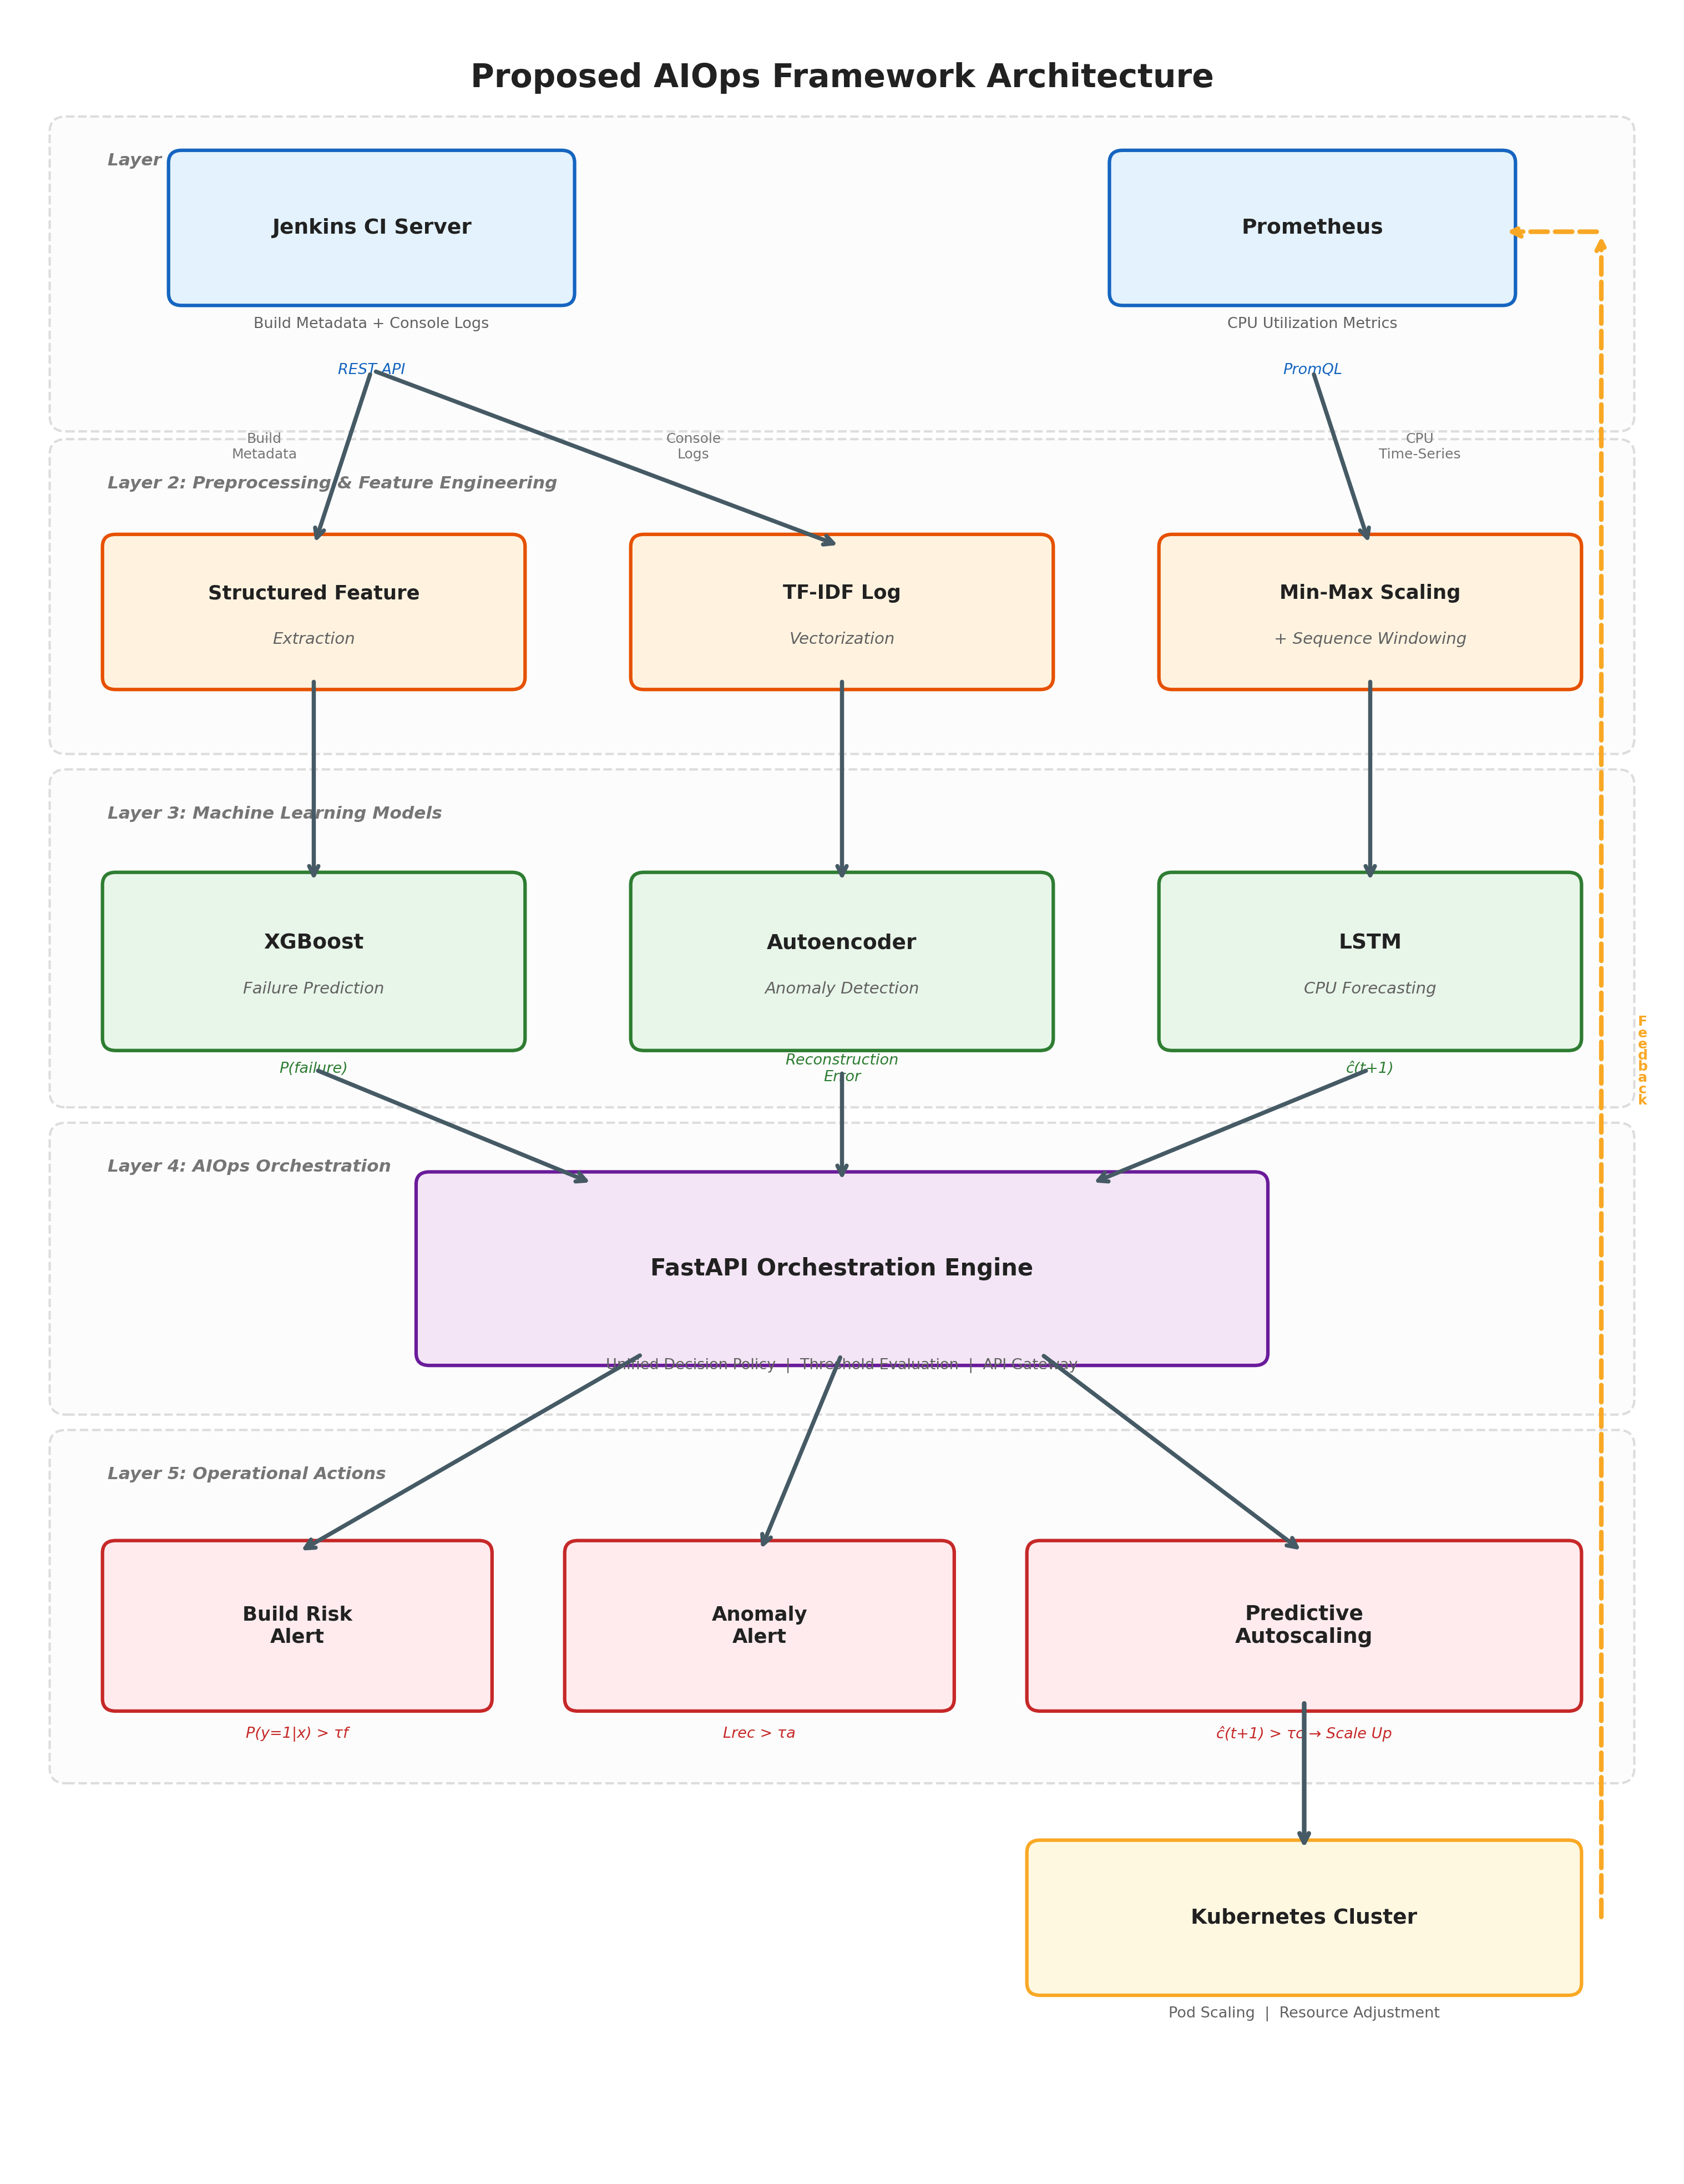
\includegraphics[width=0.85\textwidth]{architecture.png}
\caption{Proposed AIOps framework architecture. Data flows from Jenkins CI and Prometheus monitoring through preprocessing and ML inference to the FastAPI orchestration layer, which coordinates predictive autoscaling decisions via Kubernetes. The dashed feedback loop indicates continuous metric collection.}
\label{fig:architecture}
\end{figure*}

\subsection{Data Collection Layer}

Two primary operational data sources are utilized:

\textbf{1) Jenkins Build Metadata and Logs:}
Build duration, test statistics, failure counts, warning indicators, and console logs are extracted via the Jenkins REST API. Let the build dataset be represented as:

\begin{equation}
D = \{(x_i, y_i)\}_{i=1}^{N}
\end{equation}

where $x_i \in \mathbb{R}^d$ denotes a structured build feature vector, $y_i \in \{0,1\}$ indicates build success (0) or failure (1), and $N$ is the total number of builds.

\textbf{2) Prometheus CPU Metrics:}
Time-series CPU utilization metrics are collected at fixed intervals:

\begin{equation}
T = \{c_t\}_{t=1}^{M}
\end{equation}

where $c_t$ denotes CPU utilization at time step $t$ and $M$ is the total number of observations.

\subsection{Failure Prediction Using XGBoost}

Build outcome classification employs XGBoost~\cite{chen2016xgboost}, a gradient boosting framework. The prediction for build $i$ is given by:

\begin{equation}
\hat{y}_i = \sum_{k=1}^{K} f_k(x_i), \quad f_k \in \mathcal{F}
\end{equation}

where $f_k$ represents the $k^{th}$ regression tree, $\mathcal{F}$ is the space of decision trees, and $K$ is the number of boosting rounds. The objective function minimized during training is:

\begin{equation}
\mathcal{L} = \sum_{i=1}^{N} l(y_i, \hat{y}_i) + \sum_{k=1}^{K} \Omega(f_k)
\end{equation}

where $l$ is the logistic loss and $\Omega(f_k)$ is a regularization term controlling model complexity. The model outputs a failure probability $P(y=1|x)$, and a build is classified as high-risk when:

\begin{equation}
P(y=1|x) > \tau_f
\end{equation}

\subsection{Log Anomaly Detection Using TF-IDF + Autoencoder}

Console logs are first transformed into TF-IDF feature vectors:

\begin{equation}
\text{TF-IDF}(t,d) = \text{TF}(t,d) \times \log \left(\frac{N}{\text{DF}(t)}\right)
\end{equation}

Let $z \in \mathbb{R}^n$ denote the TF-IDF encoded log vector. The autoencoder learns encoder and decoder mappings:

\begin{equation}
h = \sigma(W_e z + b_e), \quad \hat{z} = \sigma(W_d h + b_d)
\end{equation}

The reconstruction loss is computed as:

\begin{equation}
\mathcal{L}_{rec} = \|z - \hat{z}\|^2
\end{equation}

An anomaly is flagged when:

\begin{equation}
\mathcal{L}_{rec} > \tau_a
\end{equation}

where $\tau_a$ is the anomaly threshold determined from the reconstruction error distribution of normal log samples~\cite{sakurada2014anomaly}.

\subsection{CPU Forecasting Using LSTM}

To enable proactive autoscaling, CPU utilization is modeled as a time-series forecasting task using an LSTM network~\cite{hochreiter1997lstm}. Given a sliding window sequence:

\begin{equation}
X_t = [c_{t-n}, c_{t-n+1}, \ldots, c_{t-1}]
\end{equation}

the LSTM predicts future CPU usage $\hat{c}_t = f(X_t)$ through gated memory operations:

\begin{equation}
f_t = \sigma(W_f [h_{t-1}, x_t] + b_f) \quad \text{(Forget Gate)}
\end{equation}

\begin{equation}
i_t = \sigma(W_i [h_{t-1}, x_t] + b_i) \quad \text{(Input Gate)}
\end{equation}

\begin{equation}
C_t = f_t \odot C_{t-1} + i_t \odot \tilde{C}_t \quad \text{(Cell State)}
\end{equation}

\begin{equation}
h_t = o_t \odot \tanh(C_t) \quad \text{(Hidden Output)}
\end{equation}

where $f_t$, $i_t$, $o_t$ are the forget, input, and output gates, respectively.

\subsection{Orchestration and Predictive Autoscaling}

A FastAPI-based orchestration layer integrates outputs from all three models: failure probability $P(y\!=\!1|x)$, anomaly score $\mathcal{L}_{rec}$, and predicted CPU $\hat{c}_{t+1}$.

Unlike the reactive Kubernetes HPA~\cite{kubernetesDocs}, scaling decisions are triggered using predicted values. The combined decision policy is:

\begin{equation}
S =
\begin{cases}
\text{Scale Up}, & \text{if } \hat{c}_{t+1} > \tau_c \\
\text{Hold}, & \text{if } P(y\!=\!1|x) > \tau_f \\
\text{Investigate}, & \text{if } \mathcal{L}_{rec} > \tau_a
\end{cases}
\end{equation}

This policy ensures that scaling actions account not only for predicted resource demand but also for pipeline stability indicators. The system forms a closed-loop architecture: data is collected from CI/CD and infrastructure sources, models generate predictions, the autoscaler adjusts resources, and updated metrics feed back into subsequent prediction cycles.

%===================================================================
\section{Experimental Setup}
%===================================================================

\subsection{Dataset Generation}

Due to the absence of publicly available CI/CD datasets containing synchronized build metadata, console log traces, and infrastructure metrics, a synthetic dataset was constructed using Python-based simulation scripts that emulate realistic CI/CD operational behavior.

\subsubsection{Build Metadata}

A total of 600 Jenkins build records were generated, each containing eight structured features: build duration, tests passed, tests failed, tests total, warning count, error count, failure count, and log length. Build outcomes followed a realistic distribution: 68.3\% SUCCESS, 22.8\% FAILURE, and 8.8\% UNSTABLE. For binary classification, FAILURE builds were assigned label~1 and all others label~0. Failure characteristics were injected probabilistically based on elevated error counts, high test failure ratios, and abnormal build durations.

\subsubsection{Console Log Data}

A corpus of 601 Jenkins console log files was generated: 464 normal logs and 137 anomalous logs (22.8\% anomaly rate). Normal logs follow consistent template patterns representing successful pipeline stages including source checkout, dependency installation, testing, and build compilation. Anomalous logs contain injected patterns including unexpected stack traces, memory overflow errors, timeout exceptions, and dependency resolution failures.

\subsubsection{CPU Time-Series Data}

A time-series of 10,080 data points was generated representing CPU utilization at one-minute intervals over a simulated seven-day period. The CPU signal is modeled as:

\begin{equation}
c_t = \mu + A \sin(\omega t) + \epsilon_t + \delta_t
\end{equation}

where $\mu$ is baseline utilization, $A$ is sinusoidal amplitude, $\epsilon_t \sim \mathcal{N}(0, \sigma^2)$ is Gaussian noise, and $\delta_t$ represents injected workload spike events.

\subsection{Model Configuration}

\subsubsection{XGBoost Configuration}

The failure prediction model was configured with 100 estimators, maximum tree depth of 4, learning rate of 0.1, and logistic loss evaluation. Class imbalance was addressed using the \texttt{scale\_pos\_weight} parameter. Performance was validated using stratified 5-fold cross-validation.

\subsubsection{Autoencoder Configuration}

The anomaly detection autoencoder was configured with layer dimensions: Input $\rightarrow$ 64 $\rightarrow$ 16 (latent) $\rightarrow$ 64 $\rightarrow$ Input, using ReLU activations and Adam optimizer. The model was trained exclusively on normal log samples. The anomaly threshold $\tau_a$ was set at the 95th percentile of reconstruction errors computed on the normal validation set.

\subsubsection{LSTM Configuration}

The CPU forecasting network consists of one LSTM layer with 50 hidden units and a single Dense output unit. A lookback window of 60 time steps and a forecast horizon of 10 time steps were used. Training was conducted for 50 epochs with Adam optimizer, MSE loss function, and early stopping to prevent overfitting.

\subsection{Data Partitioning}

For all models, datasets were split into 80\% training and 20\% testing subsets. Stratified sampling was applied for classification tasks to preserve class distribution. CPU time-series data was normalized using Min-Max scaling prior to sequence generation, yielding 10,011 input-output sequence pairs.

\subsection{Evaluation Metrics}

Classification performance was evaluated using Accuracy, Precision, Recall, F1-Score, and ROC-AUC. F1-Score was selected as the primary metric due to class imbalance. Forecasting performance was assessed using:

\begin{equation}
\text{RMSE} = \sqrt{\frac{1}{N} \sum_{i=1}^{N} (y_i - \hat{y}_i)^2}
\end{equation}

\begin{equation}
R^2 = 1 - \frac{\sum (y_i - \hat{y}_i)^2}{\sum (y_i - \bar{y})^2}
\end{equation}

\subsection{Implementation}

The framework was implemented using Python~3.13 with TensorFlow~2.20 and scikit-learn for model training. XGBoost was used for gradient boosting classification. The orchestration layer was built using FastAPI with Uvicorn. Infrastructure monitoring employed Prometheus, and the container orchestration target was Kubernetes.

%===================================================================
\section{Results and Performance Evaluation}
%===================================================================

\subsection{Failure Prediction Results}

The XGBoost classifier was evaluated on the held-out test set of 120 build records. Table~\ref{tab:classification} summarizes the classification performance. The model achieved an F1-Score of 0.964 with perfect recall (1.000), indicating that no failure cases were missed---a critical requirement in CI/CD environments where undetected failures can propagate to production deployments.

Stratified 5-fold cross-validation confirmed model stability, yielding a mean F1-Score of $0.978 \pm 0.014$ and mean ROC-AUC of $0.999 \pm 0.001$, demonstrating consistent generalization across data folds.

The confusion matrix (Fig.~\ref{fig:xgb_confusion}) shows only two false positives (stable builds predicted as failures) and zero false negatives. The ROC curve (Fig.~\ref{fig:xgb_roc}) demonstrates strong class separability. Feature importance analysis (Fig.~\ref{fig:xgb_features}) reveals that \textit{tests\_passed}, \textit{tests\_total}, and \textit{error\_count} are the most influential predictors, consistent with empirical CI failure analyses~\cite{rausch2017empirical}.

\begin{figure}[htbp]
\centering
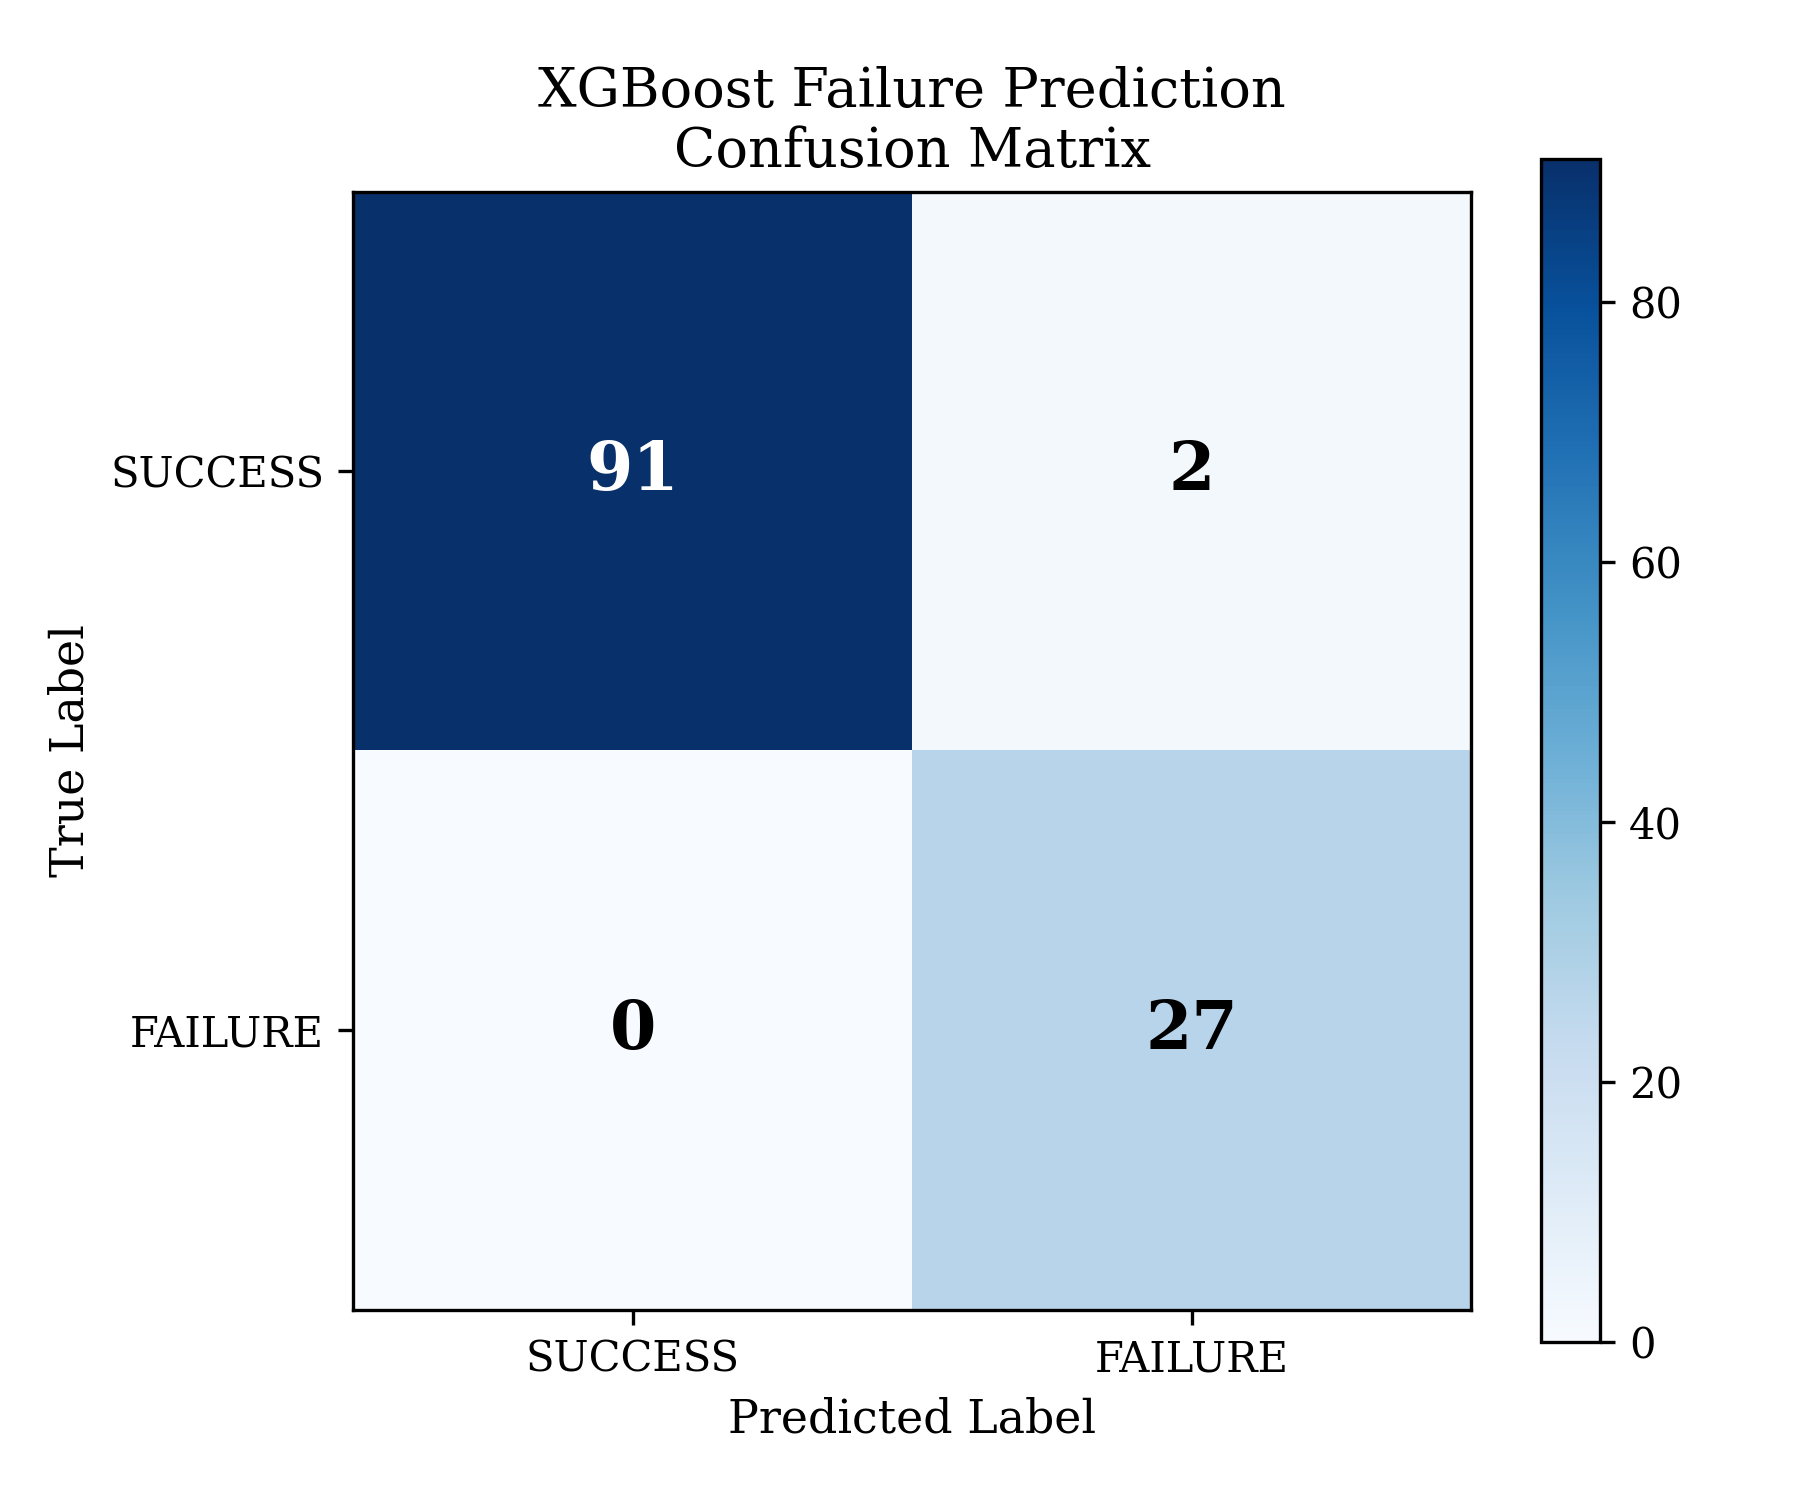
\includegraphics[width=\linewidth]{xgboost_confusion_matrix.png}
\caption{Confusion matrix for XGBoost failure prediction on 120 test builds.}
\label{fig:xgb_confusion}
\end{figure}

\begin{figure}[htbp]
\centering
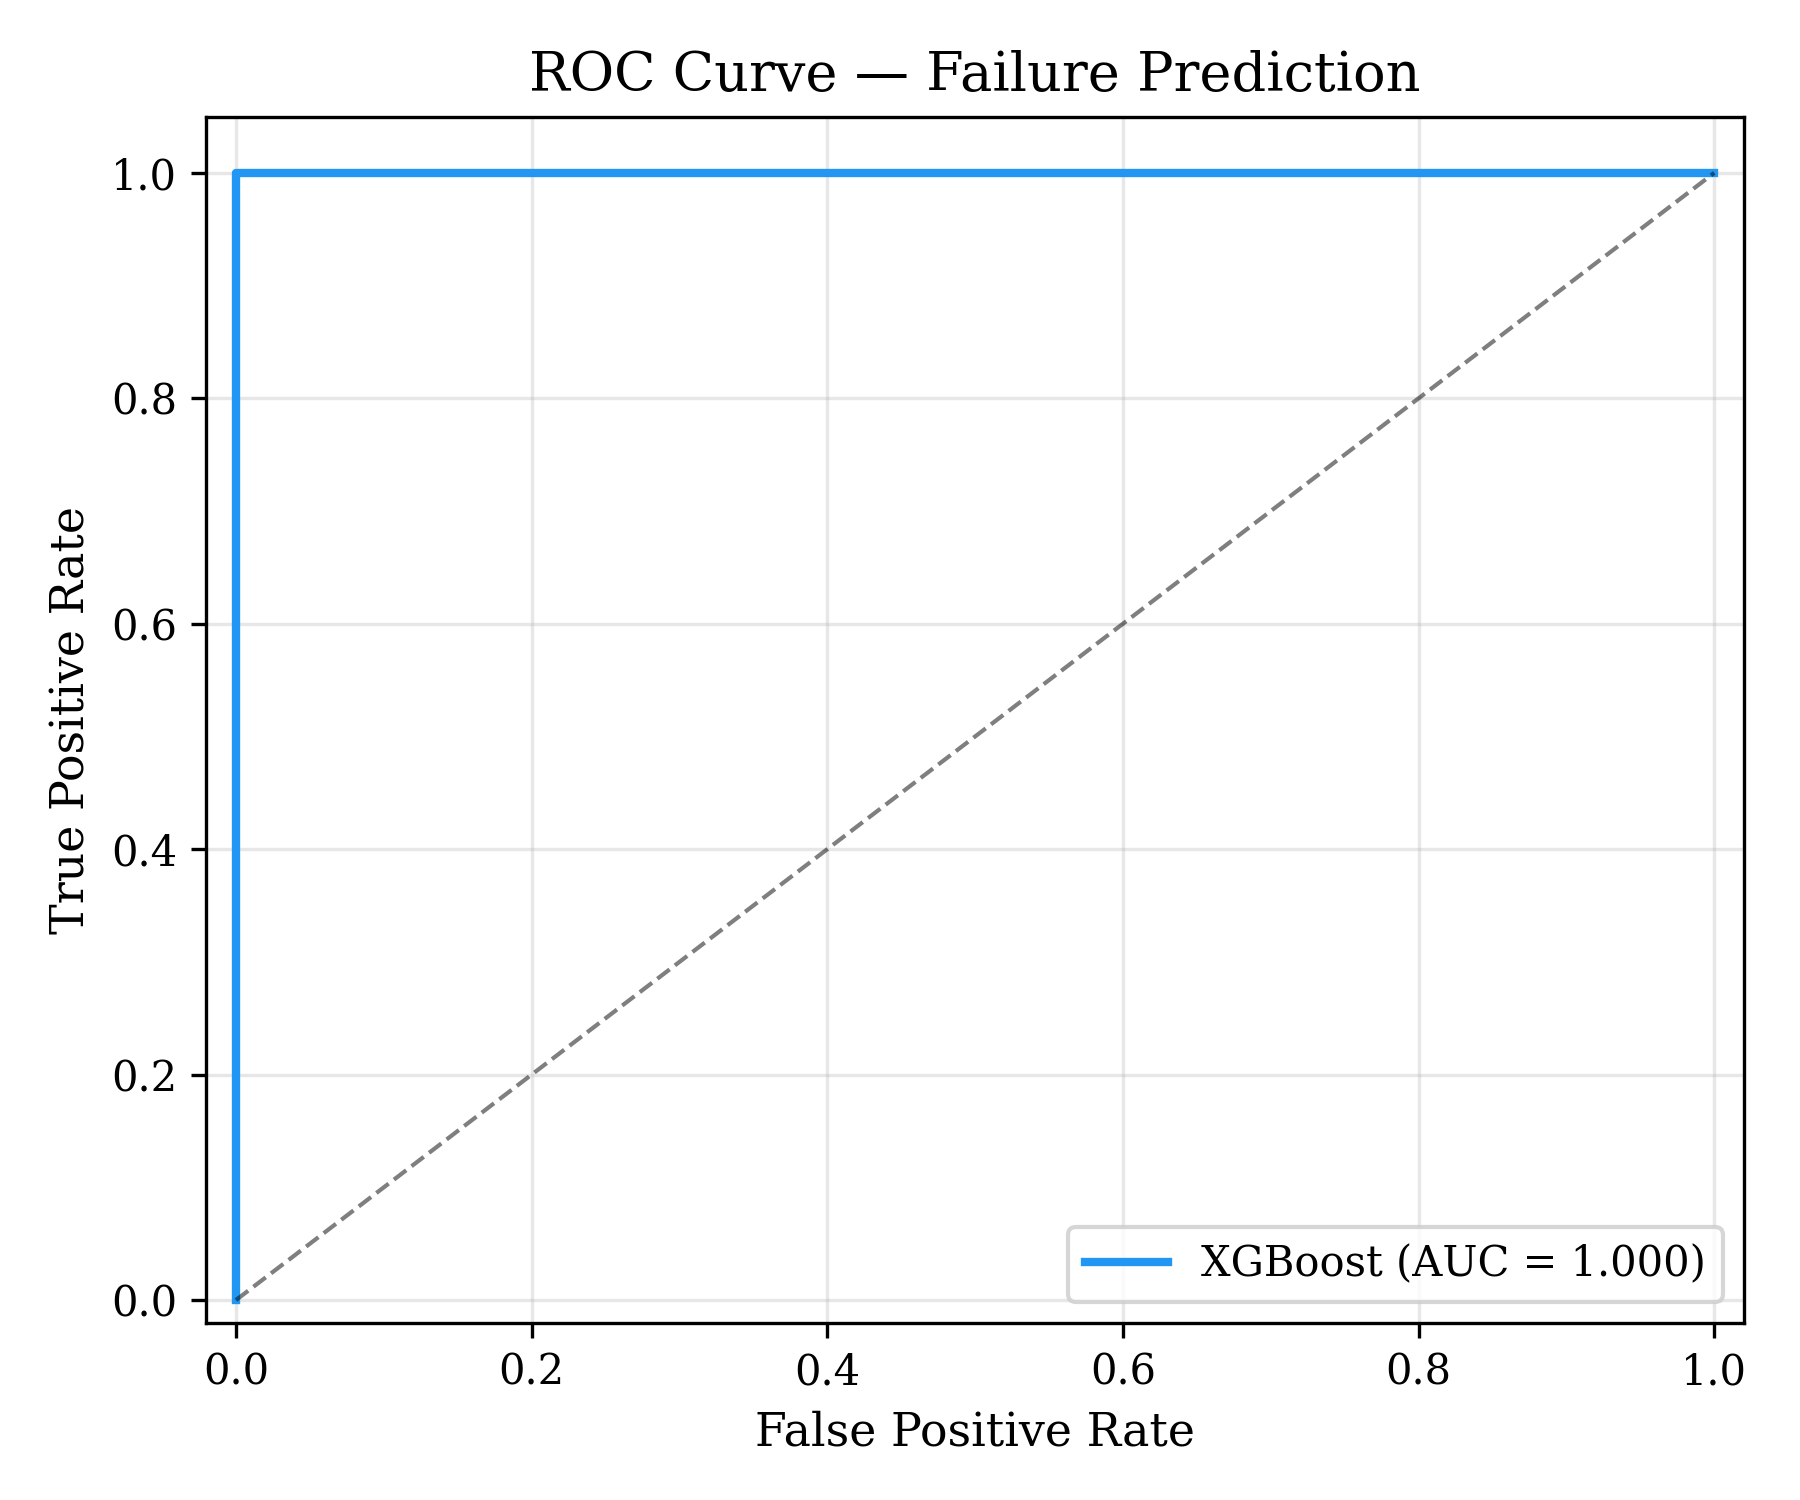
\includegraphics[width=\linewidth]{xgboost_roc_curve.png}
\caption{ROC curve for XGBoost failure prediction (AUC = 1.000).}
\label{fig:xgb_roc}
\end{figure}

\begin{figure}[htbp]
\centering
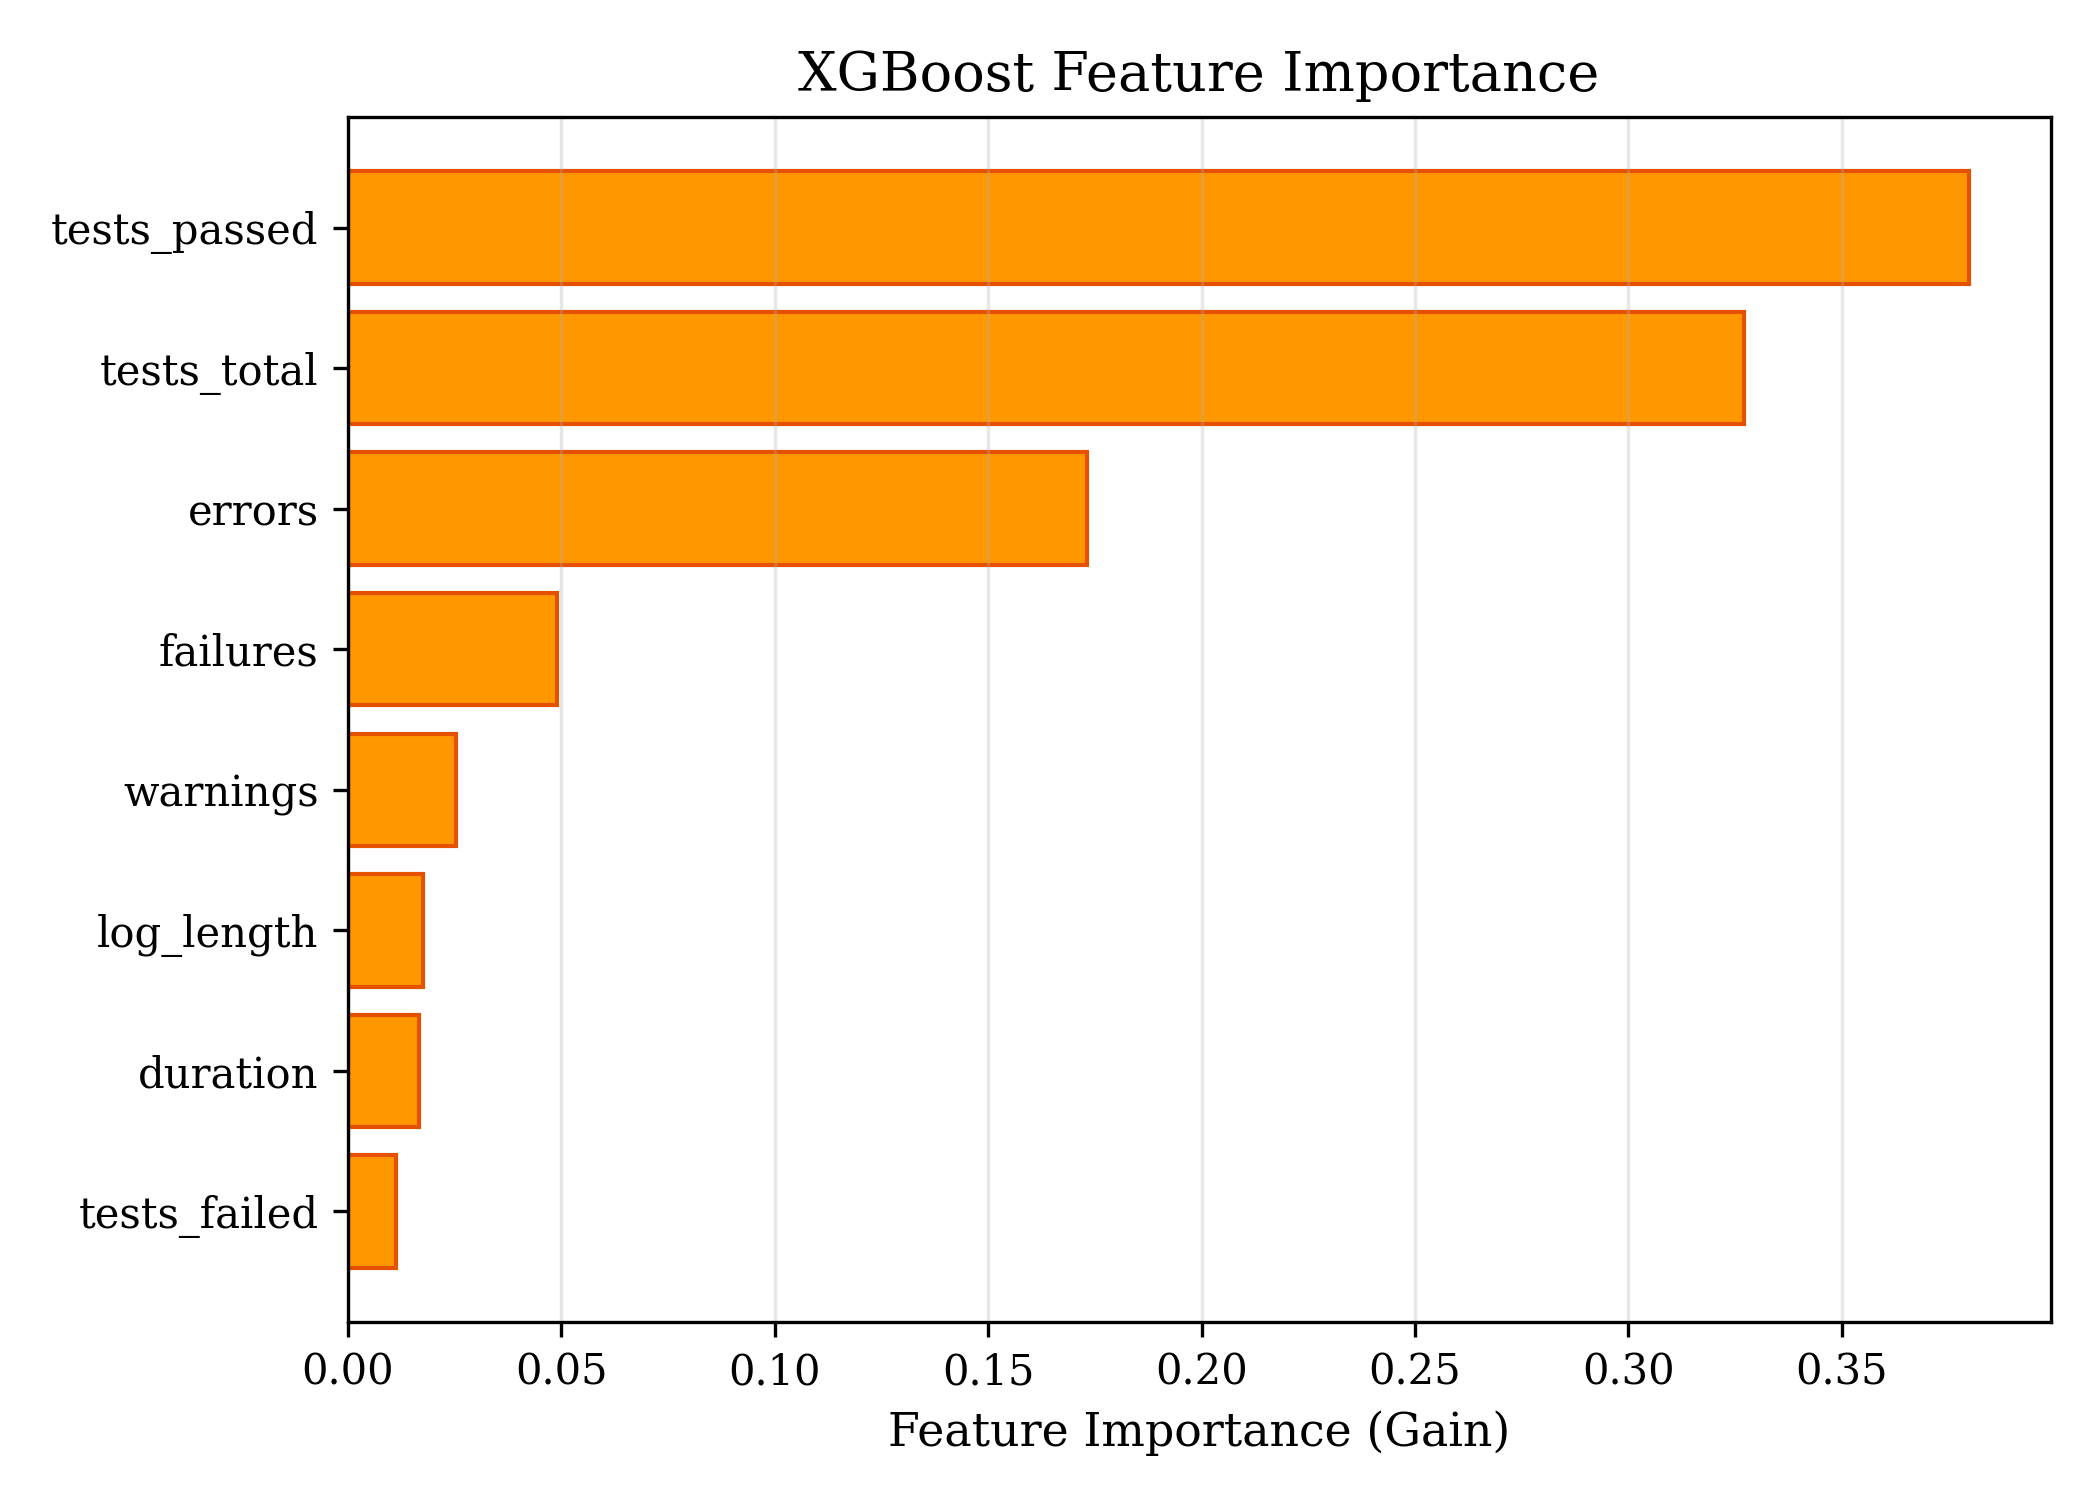
\includegraphics[width=\linewidth]{xgboost_feature_importance.png}
\caption{Feature importance ranking from the XGBoost model.}
\label{fig:xgb_features}
\end{figure}

\subsection{Log Anomaly Detection Results}

The TF-IDF + Autoencoder model was evaluated on the held-out log test set. Table~\ref{tab:classification} presents the results. The model achieved an F1-Score of 0.918 with perfect recall, successfully identifying all injected anomalies.

The reconstruction error distribution (Fig.~\ref{fig:ae_error}) shows clear separation between normal and anomalous samples, validating the threshold-based detection strategy. The confusion matrix (Fig.~\ref{fig:ae_confusion}) reveals that false positives (normal logs classified as anomalous) constitute the primary error mode, a consequence of the conservative threshold selection at the 95th percentile~\cite{sakurada2014anomaly}. This configuration is operationally appropriate, as missed anomalies (false negatives) carry higher risk than false alerts in CI/CD environments.

\begin{figure}[htbp]
\centering
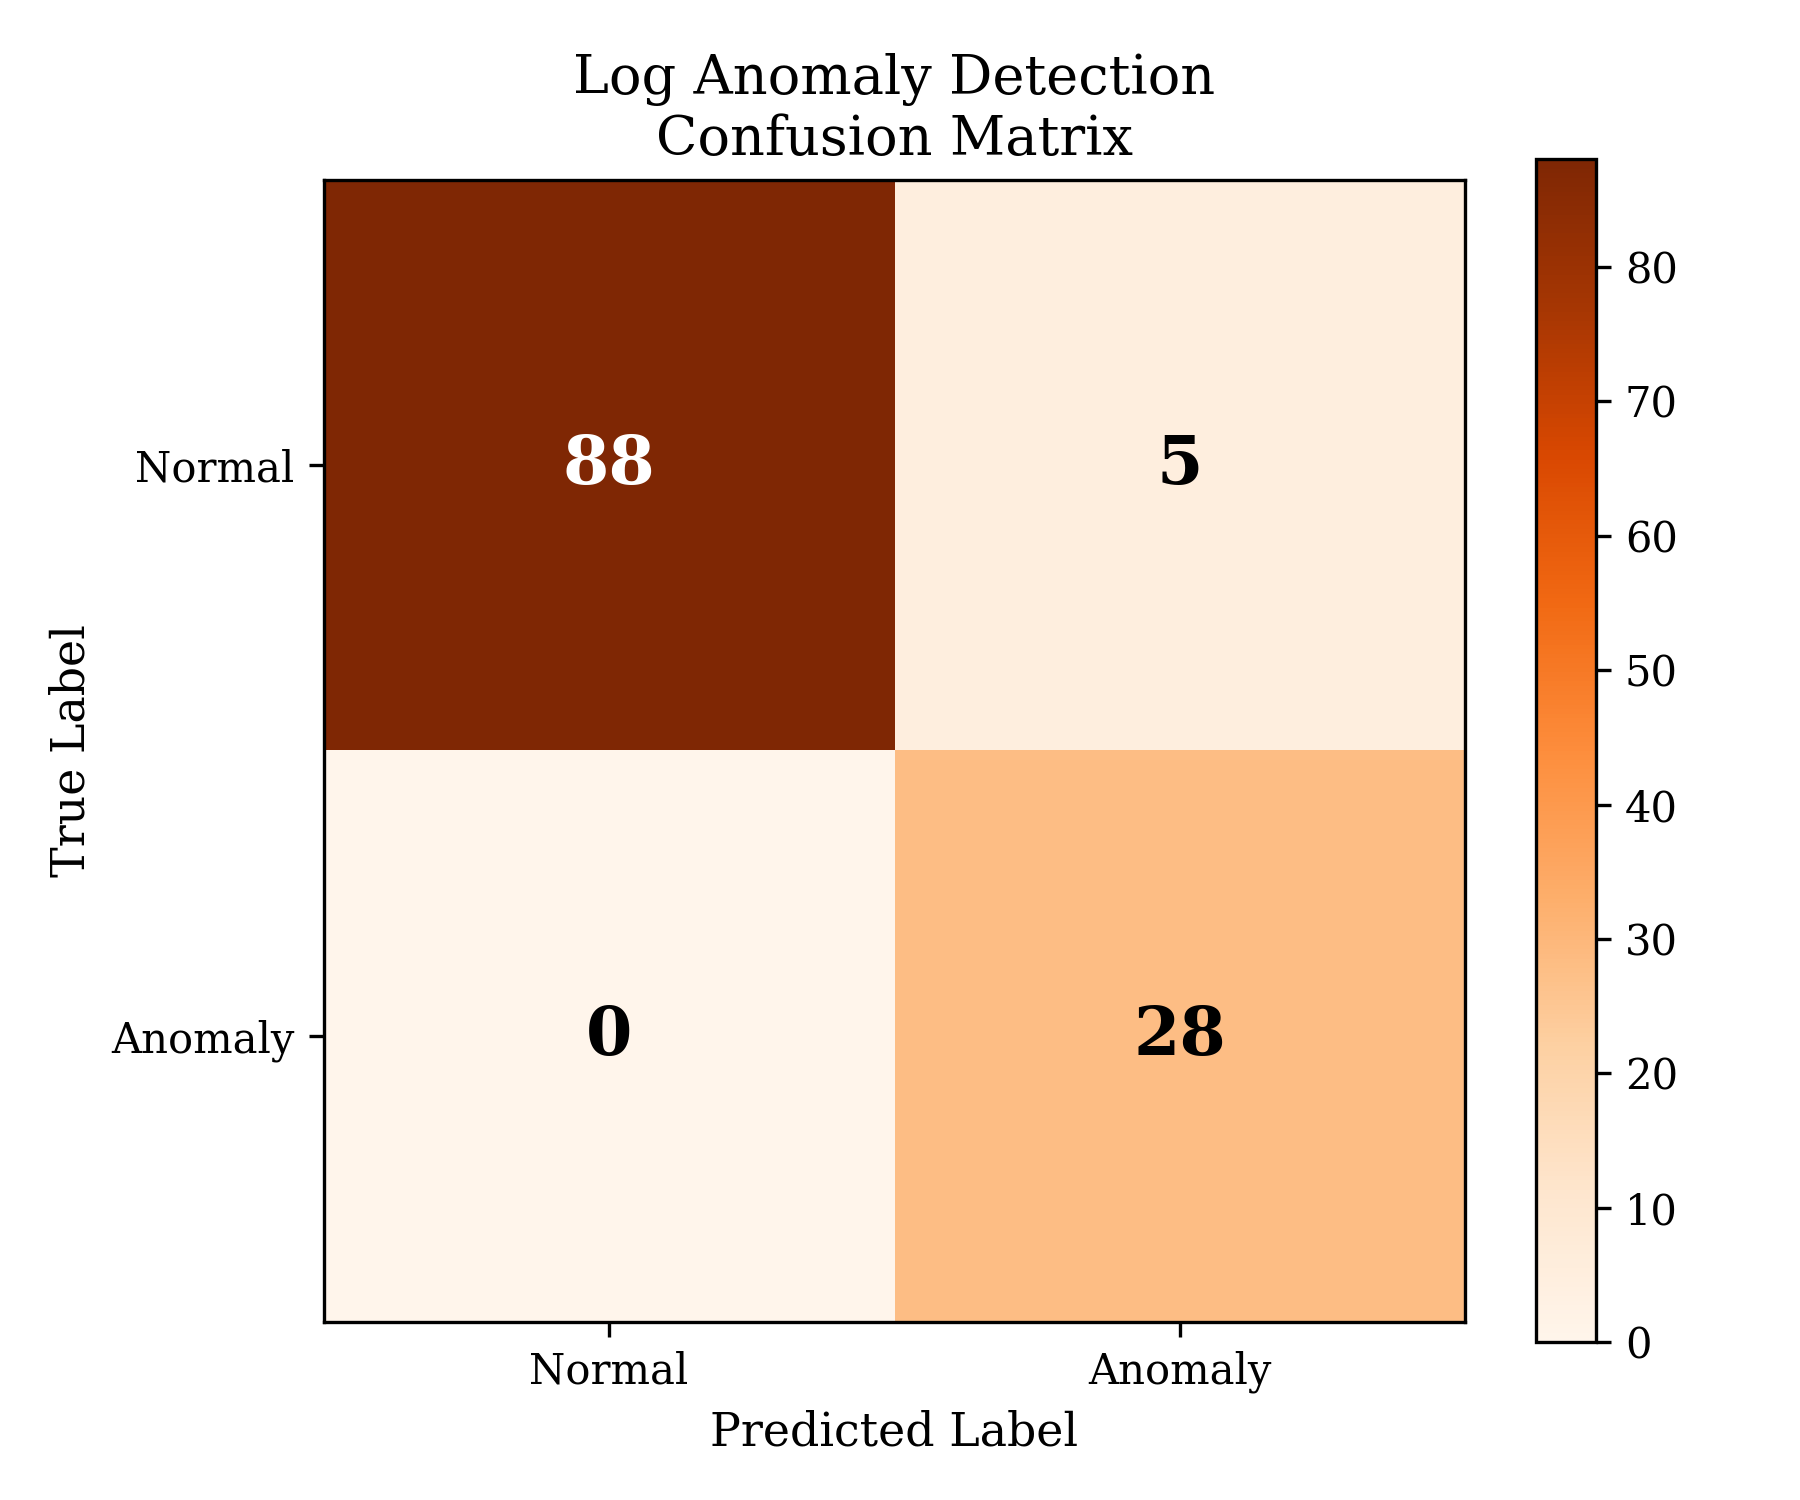
\includegraphics[width=\linewidth]{anomaly_confusion_matrix.png}
\caption{Confusion matrix for autoencoder-based log anomaly detection.}
\label{fig:ae_confusion}
\end{figure}

\begin{figure}[htbp]
\centering
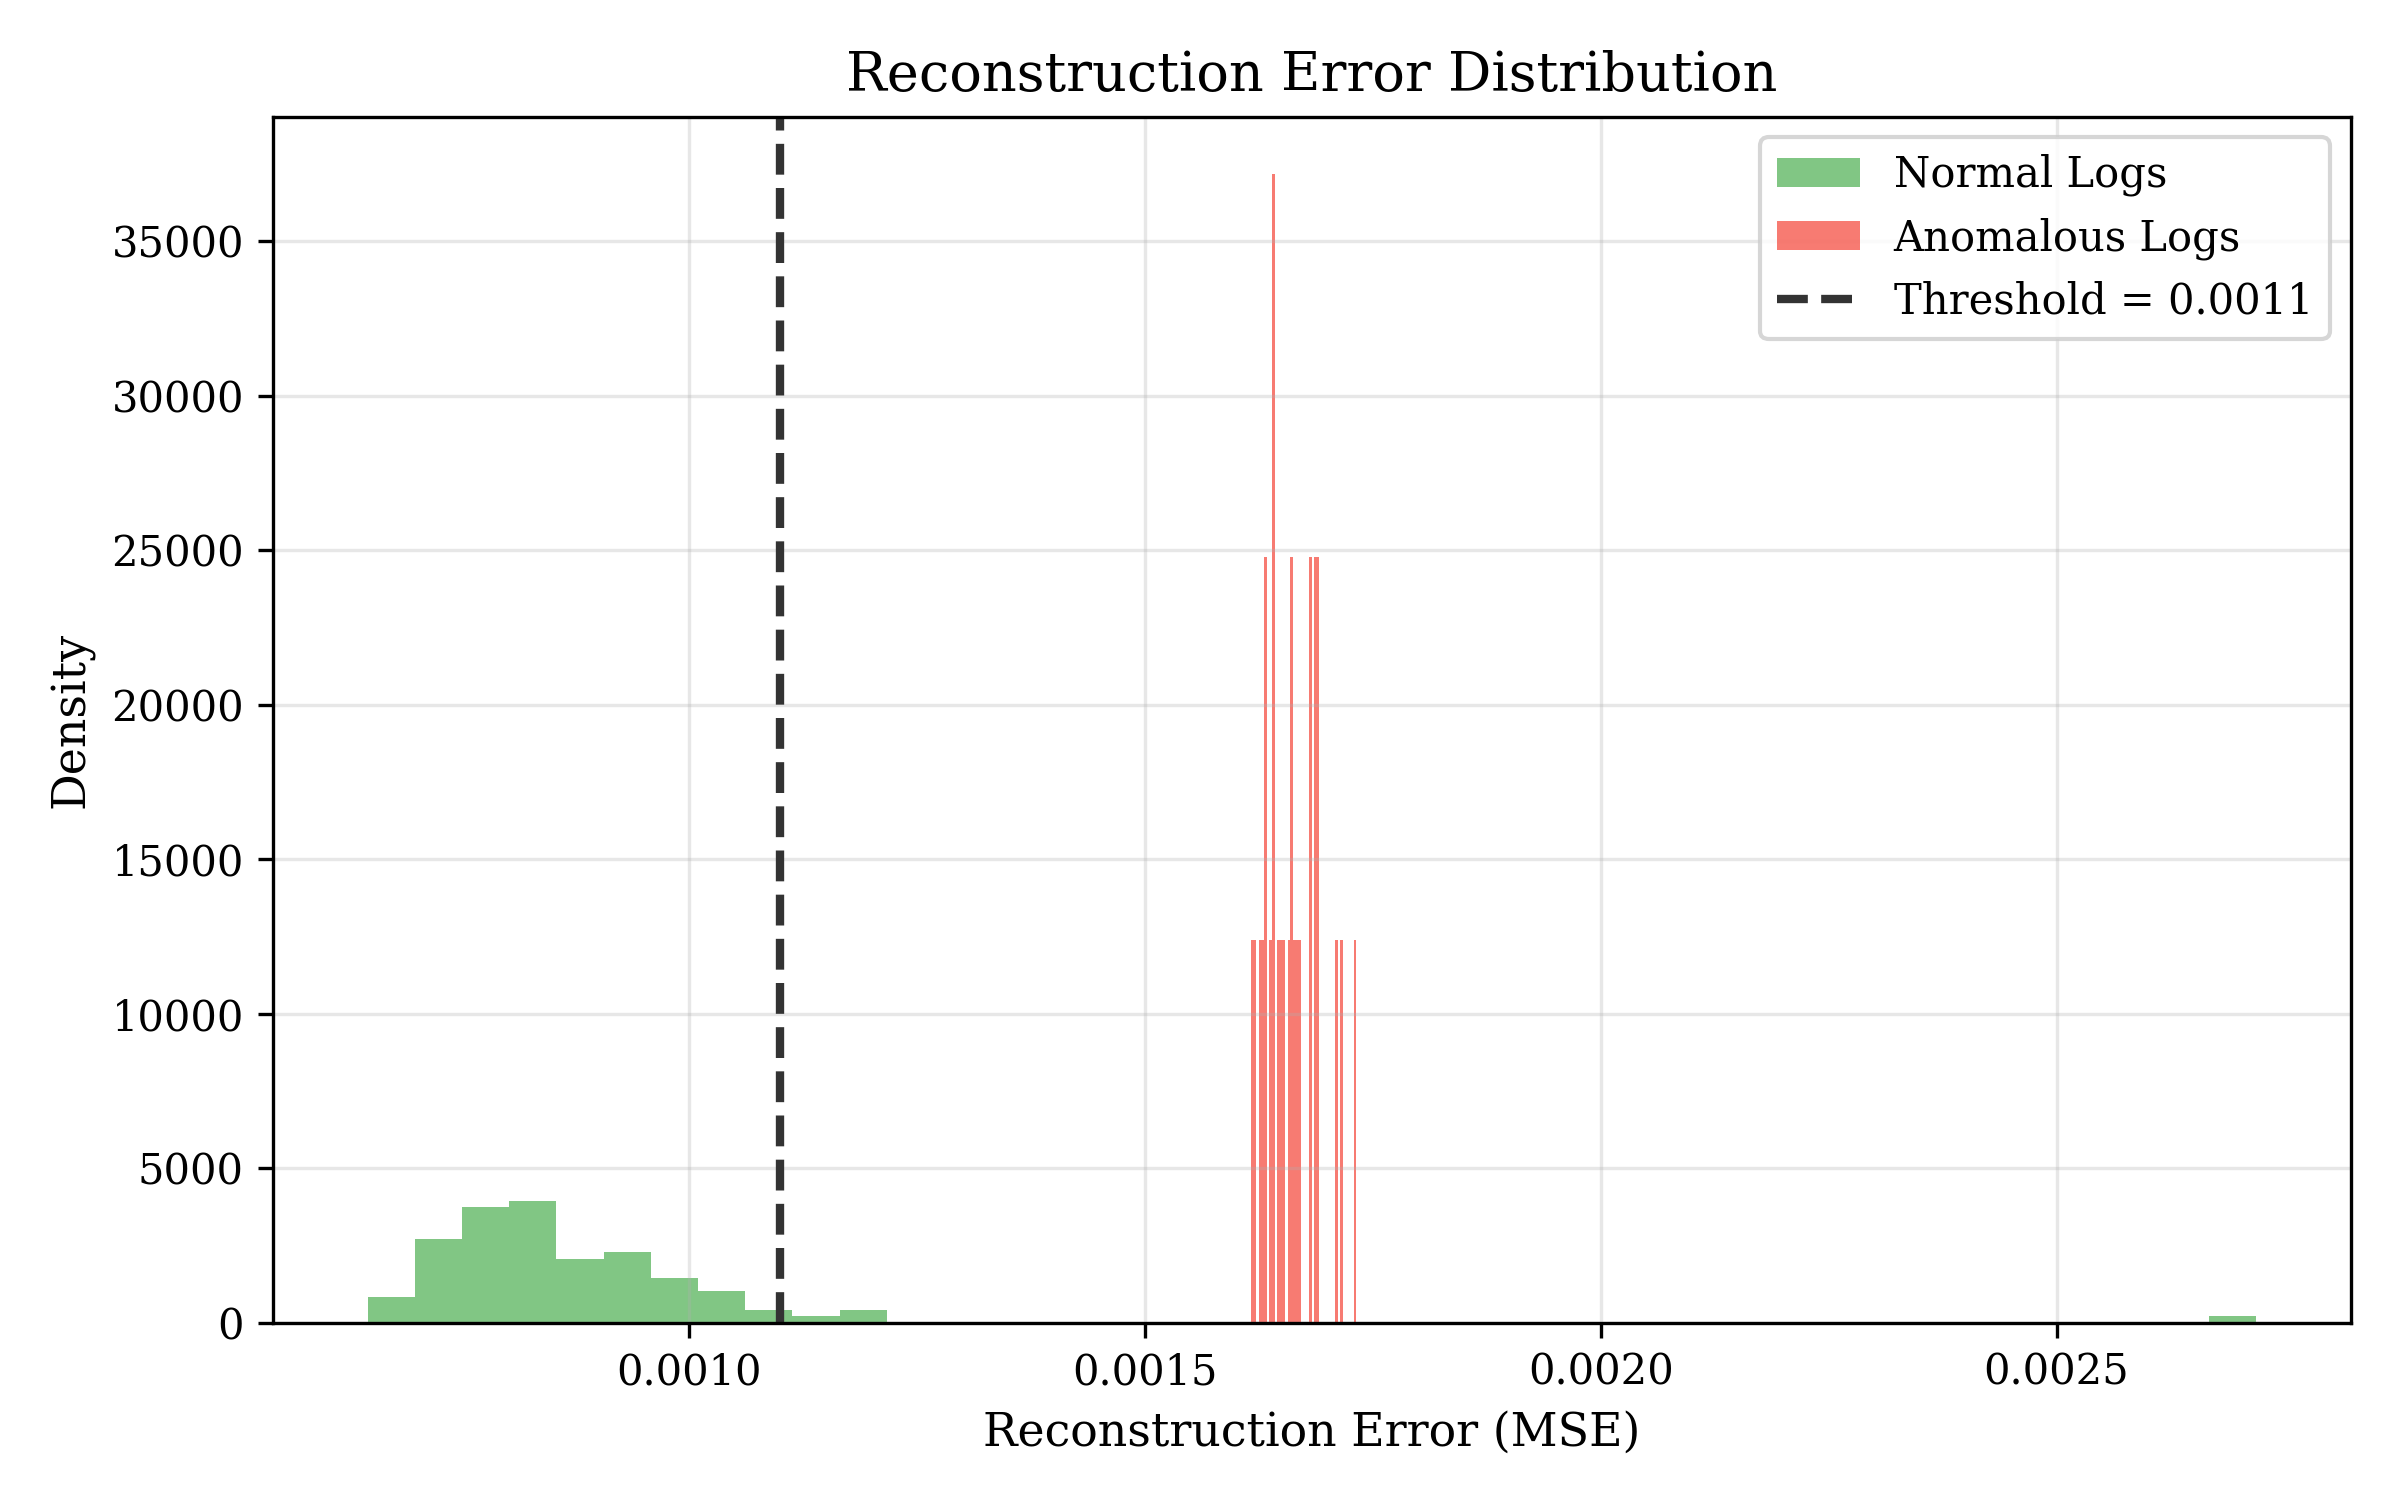
\includegraphics[width=\linewidth]{anomaly_error_distribution.png}
\caption{Reconstruction error distribution. Clear separation is observed between normal and anomalous samples. The dashed line indicates the detection threshold $\tau_a$.}
\label{fig:ae_error}
\end{figure}

\subsection{CPU Forecasting Results}

The LSTM model was evaluated on approximately 2,000 held-out test sequences derived from the 10,080-point CPU time-series. Table~\ref{tab:forecasting} presents the forecasting metrics. The model achieved an RMSE of 0.071 and MAE of 0.044, indicating that predictions deviate from actual utilization by approximately 4.4 percentage points on average.

The $R^2$ value of 0.435 indicates the model captures a moderate proportion of variance, reflecting the inherent stochasticity of the synthetic workload signal including injected noise and spike events. Figure~\ref{fig:lstm_prediction} illustrates the model's ability to track dominant temporal trends while smoothing high-frequency noise.

\begin{figure}[htbp]
\centering
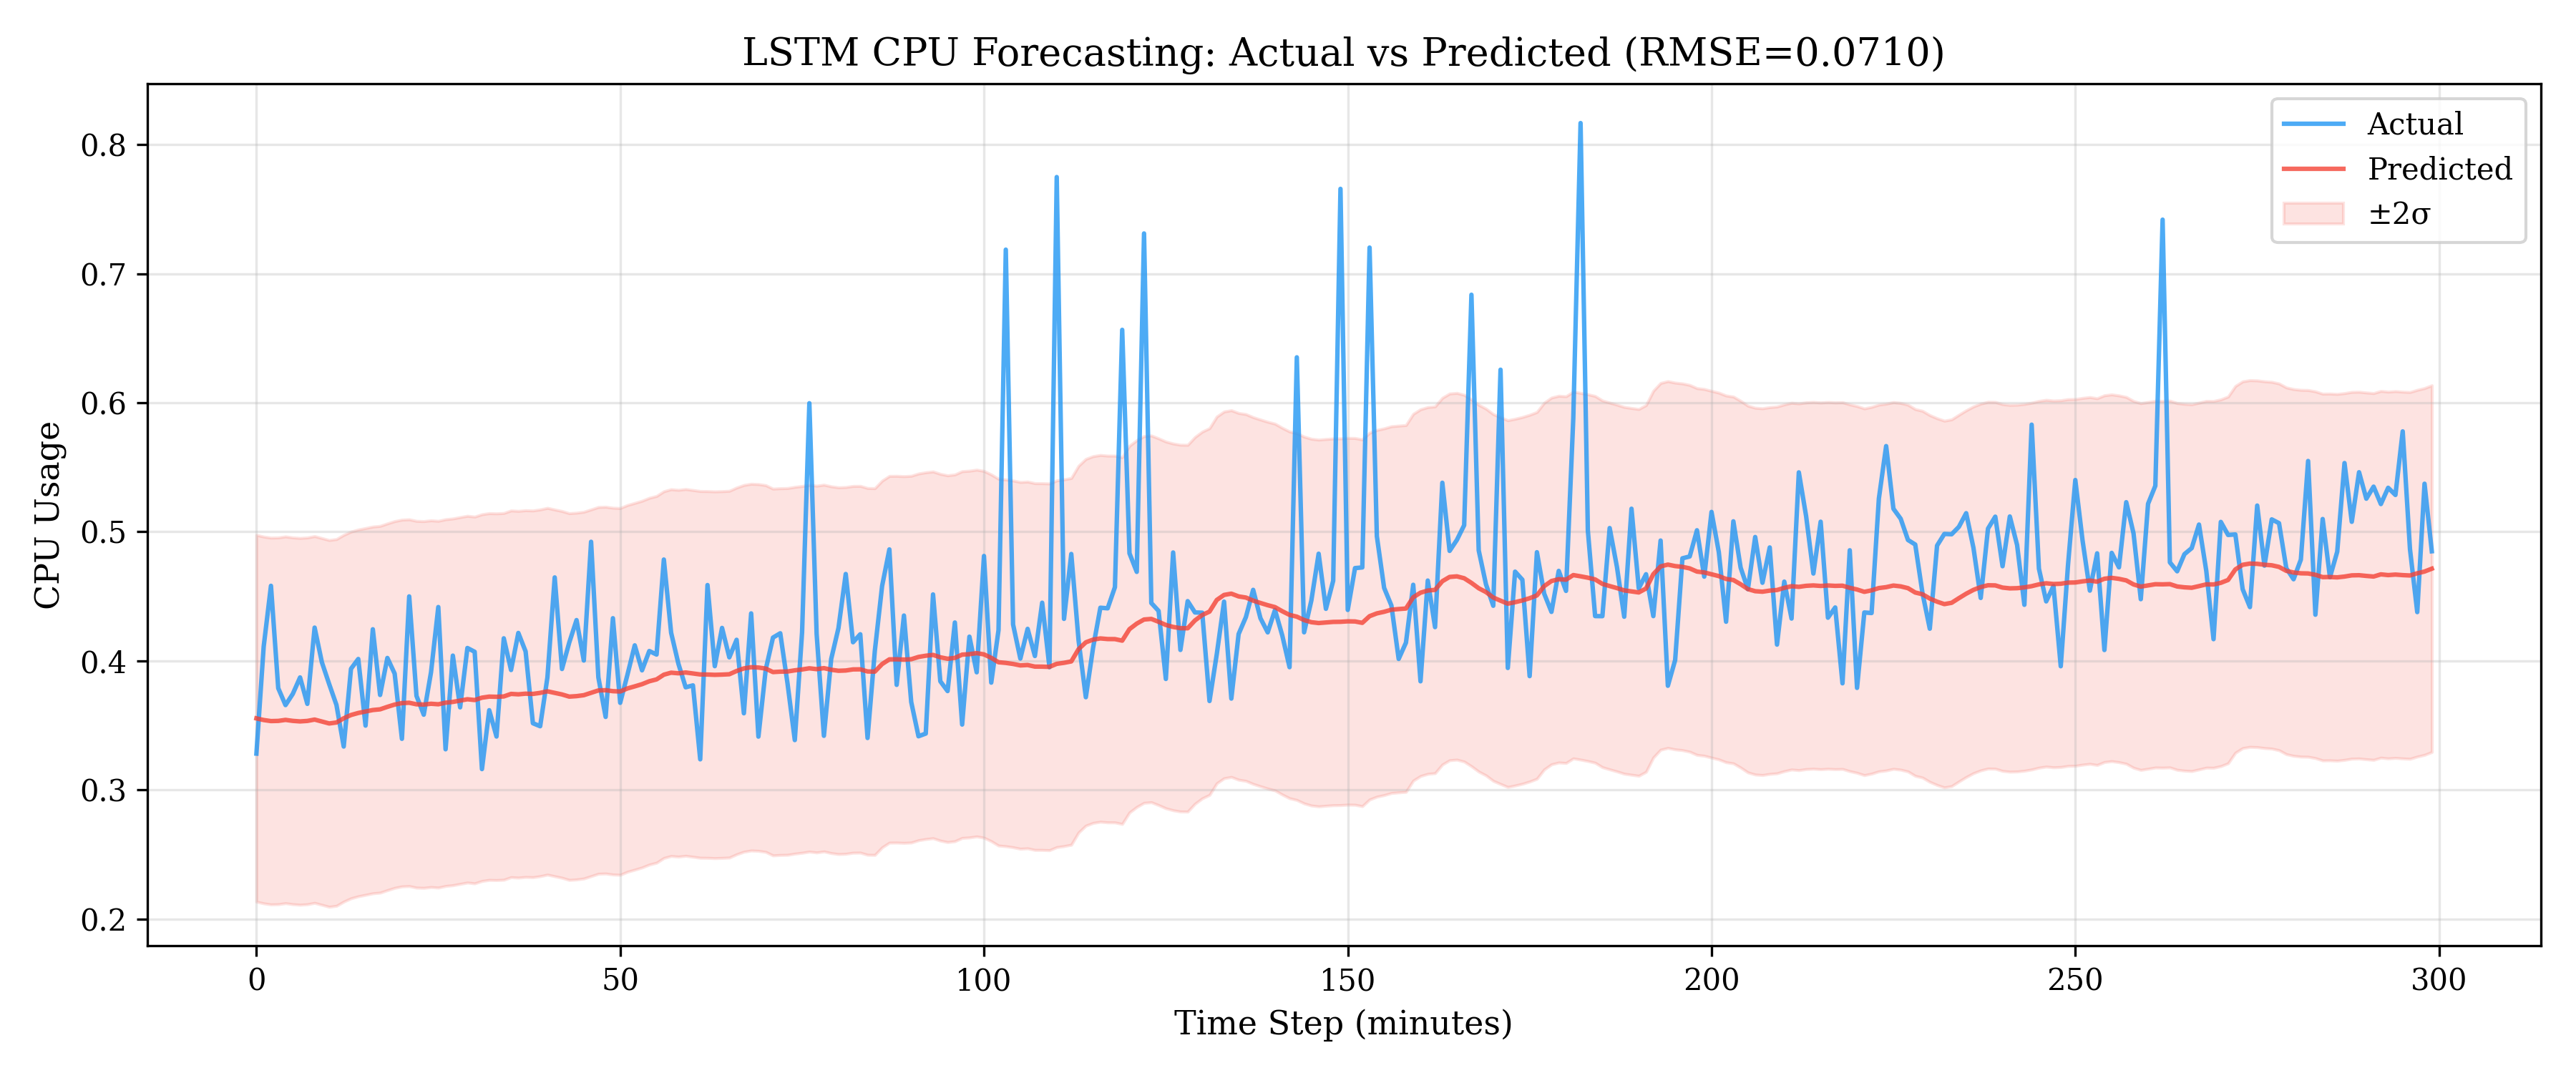
\includegraphics[width=\linewidth]{lstm_actual_vs_predicted.png}
\caption{Actual vs.\ predicted CPU utilization using the LSTM forecasting model.}
\label{fig:lstm_prediction}
\end{figure}

\subsection{Consolidated Performance Summary}

\begin{table}[htbp]
\caption{Classification Performance: Failure Prediction and Anomaly Detection}
\centering
\begin{tabular}{lcc}
\toprule
\textbf{Metric} & \textbf{XGBoost} & \textbf{Autoencoder} \\
 & \textbf{(Failure Pred.)} & \textbf{(Anomaly Det.)} \\
\midrule
Accuracy & 0.983 & 0.959 \\
Precision & 0.931 & 0.848 \\
Recall & 1.000 & 1.000 \\
F1-Score & 0.964 & 0.918 \\
ROC-AUC & 1.000 & 0.989 \\
\bottomrule
\end{tabular}
\label{tab:classification}
\end{table}

\begin{table}[htbp]
\caption{LSTM CPU Forecasting Performance}
\centering
\begin{tabular}{lc}
\toprule
\textbf{Metric} & \textbf{Value} \\
\midrule
MSE & 0.0050 \\
RMSE & 0.0710 \\
MAE & 0.0436 \\
MAPE & 9.56\% \\
$R^2$ & 0.435 \\
\bottomrule
\end{tabular}
\label{tab:forecasting}
\end{table}

\subsection{Discussion}

The experimental results demonstrate that the proposed AIOps framework achieves strong predictive performance across all three operational dimensions. Both classification models achieve perfect recall (1.000), prioritizing the detection of adverse events---build failures and log anomalies---at the cost of modest false positive rates. This design choice aligns with operational requirements in CI/CD environments, where missed failures carry substantially higher cost than false alerts~\cite{dang2019aiops}.

The XGBoost failure predictor achieved near-perfect class separability (ROC-AUC = 1.000), driven by the controlled nature of the synthetic dataset where failure indicators are injected with clear feature signatures. The autoencoder-based anomaly detector achieved an ROC-AUC of 0.989, demonstrating effective learned representation of normal log behavior and sensitivity to injected anomaly patterns.

The LSTM forecasting module captures temporal workload trends sufficiently to support proactive scaling decisions, with the moderate $R^2$ reflecting the challenge of predicting stochastic workload components including sudden spikes. The RMSE of 0.071 represents an operationally useful level of prediction accuracy for threshold-based autoscaling decisions.

Compared to traditional reactive monitoring, where failures and resource overloads are addressed only after occurrence, the proposed framework provides advance operational intelligence across build stability, log health, and resource demand. The integration of these signals through a unified orchestration layer represents a step toward the closed-loop AIOps architectures advocated by Dang et al.~\cite{dang2019aiops} and Notaro et al.~\cite{notaro2021aiops}.

%===================================================================
\section{Challenges and Limitations}
%===================================================================

\subsection{Synthetic Dataset Constraints}

The evaluation was conducted on synthetically generated data. While controlled simulation enables reproducibility and structured experimentation, it may not fully capture the complexity of production CI/CD environments, which exhibit noisy log streams, multi-service dependency failures, and infrastructure-level disruptions. The near-perfect ROC-AUC in failure prediction is partly attributable to the controlled separability of synthetic data. Production deployment would likely yield reduced performance due to noisier feature distributions.

\subsection{Concept Drift}

CI/CD pipelines evolve through frequent codebase modifications, updated test suites, and infrastructure changes, introducing concept drift where statistical properties of input features shift over time. Models trained on historical data may degrade without periodic retraining. Future deployments must incorporate drift detection mechanisms and scheduled or incremental retraining strategies.

\subsection{Scalability Considerations}

Although the FastAPI orchestration layer provides modular integration, real-time inference at enterprise scale may introduce latency constraints. Organizations executing thousands of daily builds would require horizontally scaled model serving infrastructure with asynchronous inference capabilities. Advanced log models leveraging transformer architectures~\cite{le2022log} may improve detection but impose significant computational overhead compared to the lightweight autoencoder approach employed here.

\subsection{Forecasting Limitations}

The LSTM model effectively captured long-term workload trends but exhibited reduced sensitivity to abrupt spike events caused by batch merges or scheduled regression tests. Incorporating exogenous variables such as commit frequency, build queue length, and deployment schedules may enhance forecasting robustness.

\subsection{Operational Integration Risks}

Predictive autoscaling introduces decision complexity. Improperly calibrated thresholds may cause over-provisioning (increased cloud costs), under-provisioning (SLA violations), or resource oscillation. Careful policy tuning and validation are required before production deployment.

%===================================================================
\section{Conclusion and Future Work}
%===================================================================

This paper presented a unified AIOps framework for intelligent CI/CD pipeline optimization, integrating failure prediction, log anomaly detection, and predictive autoscaling within a single closed-loop operational architecture. The XGBoost failure predictor achieved an F1-Score of 0.964 with zero false negatives. The TF-IDF and autoencoder-based anomaly detector identified abnormal log patterns with an F1-Score of 0.918. The LSTM-based forecasting model captured temporal workload trends with an RMSE of 0.071, enabling proactive scaling beyond the capabilities of reactive Kubernetes HPA mechanisms~\cite{kubernetesDocs}.

The primary contribution lies in the holistic integration of supervised, unsupervised, and time-series models within a closed-loop orchestration layer. By combining failure signals, anomaly scores, and infrastructure forecasts, the framework enables coordinated operational decisions that improve reliability and resource efficiency.

Although evaluation was conducted on synthetic data, the results demonstrate the feasibility and potential impact of integrated AIOps strategies for CI/CD environments. Future work will focus on validating the framework in production CI/CD pipelines with real operational data. Incorporating transformer-based log embeddings~\cite{le2022log}, drift-aware adaptive learning pipelines, and reinforcement learning-based autoscaling policies may further enhance system intelligence. Extending the framework to balance performance, cost, and energy efficiency represents a promising direction for sustainable DevOps automation.

\bibliographystyle{IEEEtran}
\bibliography{aiops_cicd_refs}

\end{document}
